\chapter{Previous Work}\label{chap:litReview}

Laureti et al. \cite{laureti2006information} introduced iterative filtering as an aggregation method. It set out to appropriate some methods for examining complex networks that had been looked into within the physics community and apply them to scoring systems on the internet. They found that a reciprocal variance method was highly effective at reducing the effects of systemic errors and collusion. They were primarily concerned with the use case of voting on the internet and demonstrated how the reciprocal variance weighting system described in equation \ref{eq:negRecip} would reduce the effectiveness of a cheater the more they cheated, as demonstrated in figure \ref{fig:recipCheating}.

\begin{figure}[H]
    \centering
    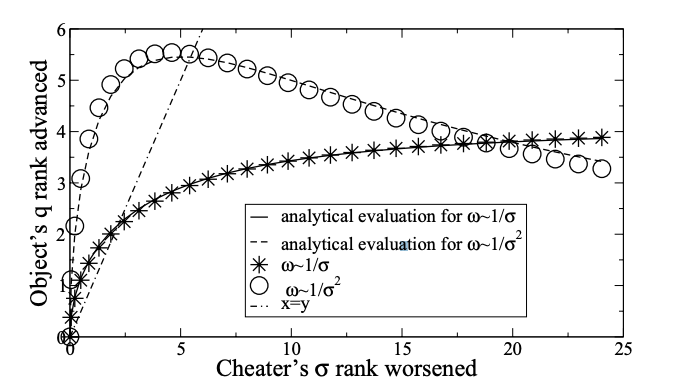
\includegraphics{Figures/recipCheating.png}
    \caption[Relationship between voters accuracy and marginal effect of their vote on an object]{Relationship between voters accuracy and marginal effect of their vote on an object, from \textcite{laureti2006information}.}
    \label{fig:recipCheating}
\end{figure}

De Kerchoove and Van Dooren \cite{de2007iterative} went on to improve applicability of the algorithm by examining a variety of weighting functions, including the affine method defined recursively in equations \ref{eq:affine} and \ref{eq:affineBase}, in order to account for predictable human behaviours, such as clumsiness or dishonesty. 
They further examine iterative filtering as it could be a applied to dynamical systems, that is one where there is a constant flow of ratings. The examination of is particularly relevant to the topic of this thesis, however they do not examine the case of ratings degradation to preempt changes in quality over time, an issue likely to be critical to this project.  Their experiments validated a slightly modified\footnote{Limiting the number of iterations rather than continuing until convergence was found to provide adequate results while still allowing for rapid updates of ratings.} reciprocal variance method for use within dynamical systems. They also performed a number of experiments to show that IF is very useful for cheater detection. 

\begin{align}
    \tilde{u}^{(n)} &= \sum\limits_{i \in R}\frac{\frac{r_i}{|r_i-\tilde{u}^{(n-1)}|+\epsilon}}{\sum\limits_{j\in R} \frac{1}{|r_j-\tilde{u}^{(n-1)}|+\epsilon}} \label{eq:affine} \\
    \tilde{u}^{(0)} &= \frac{\sum\limits_{i\in R} r_i}{|R|}\label{eq:affineBase}
\end{align}


De Kerchoove and Van Dooren's \cite{de2010iterative} second paper in the area went into great detail about the various quadratic and affine weighting methods available and demonstrated the validity of all of them. The paper goes on to examine the effects of a very sparse voting matrix and and demonstrates the effectiveness of modified techniques in aggregating such information.

These techniques will likely be very useful when it comes to designing a system that can handle recommendations about small-cap stocks which are typically under-covered by analysts. By ensuring that the method chosen is valid for all securities, the system could be more easily expanded and automated for a larger range of financial products.

Zhou et al. \cite{zhou2011robust} added to the current set of quadratic and affine weighting paradigms by designing a system that used the correlation of a user's rating and an objects rating to enhance it's assignment of weights. This method was shown to be very effective against other forms of IF on IMDB and Netflix Prize data.

Ignjatovic et al. \cite{ignjatovic2009computing} specifically examined the case of multiple assessors marking assignments and considered specifically the cases that a case of systemic bias as well as providing methods to adjust for issues that are likely to be encountered, such as a small number of markers per assessment.

This naturally flows over into the problem at hand where the number and frequency of recommendations is likely to correlate quite strongly with the market cap of the stock and thus a system may need to take issues like this into account when aggregating ratings in order to provide more valid recommendations.

Rezvani et al. \cite{rezvani2018provenance} examined several significant modifications and addons to other methods and looked into specifically:
\begin{description}
    \item[Provenance] Many factors can potentially be used to inform trustworthiness beyond simply the votes that are cast. External factors such as independence or even size of a research house could factor into the accuracy of its ratings and thus such information should be used in the model.
    \item[Multi-Dimensional Reputation] The paper proposed having a main trust score and having multiple dimensions be some factor of that trust score.
\end{description}